\documentclass[12pt]{article}
\usepackage[swedish]{babel}
\usepackage[T1]{fontenc}{
\usepackage[utf8]{inputenc}
\usepackage{amssymb}
\usepackage{amsmath}
\usepackage{amsfonts}
\usepackage{url,graphicx,tabularx,array,geometry,color,float,placeins}
\usepackage{tikz}
\usetikzlibrary{shapes, arrows, 3d, decorations}
\setlength{\parskip}{1ex} %--skip lines between paragraphs
\setlength{\parindent}{0pt} %--don't indent paragraphs
%\setcounter{secnumdepth}0}

\newcommand{\sspan}[1]{\mathrm{span}\left\{#1\right\}}
\newcommand{\ima}[1]{\mathrm{Im}\; #1}

%\linespread{2} %-- Uncomment for Double Space
\begin{document}
\begin{titlepage}
\author{Martin Biel \\ \texttt{mbiel@kth.se}}
\title{EL1000 - Reglerteknik, allmän kurs \\ \Large Övning 1}
\date{31 augusti 2016}
\end{titlepage}

\tikzstyle{block} = [draw, rectangle, thick, minimum height=3em, minimum width=6em, align=center, text width=2cm, top color=white, bottom color=white!85!black]
\tikzstyle{input} = [coordinate]
\tikzstyle{output} = [coordinate]
\tikzstyle{tmp} = [coordinate]
\tikzstyle{sum} = [draw, circle, node distance=1cm]
\tikzstyle{wire} = [->,thick]
\tikzstyle{lab} = []
\tikzstyle{laba} = [lab, label distance=0cm]
\tikzstyle{labb} = [lab, label distance=0.5em]
\tikzstyle{split} = [fill,black,circle,inner sep=0.03cm]

\maketitle

\section*{Introduktion}

Reglerteknik - Berör analys och styrning av dynamiska system \\\\
Typiska problem:
\begin{itemize}
	\item \textbf{Servoproblemet} - Styr ett system till ett givet tillstånd 
	\item \textbf{Regulatorproblemet} - Bibehåll ett tillstånd under inverkan av störning
\end{itemize}

\textbf{EL1000}
\begin{itemize}
\item Klassisk reglerteknik
  \begin{itemize}
  \item Analys: I frekvensplanet via Laplace-transformering
  \item Reglering: Återkoppling från mätsignal $\rightarrow$ slutet system
  \item Verktyg: Rotort, Nyquistkurvan, Bodediagram
  \item PID-regulatorn
  \end{itemize}
\item Modern styrteori
  \begin{itemize}
  \item Analys: I tidsdomänen på tillståndsform
  \item Reglering: Tillståndsåterkoppling, polplacering, LQ
  \item Koncept: Stabilitet, styrbarhet, observerbarhet
  \end{itemize}
\item Även
  \begin{itemize}
  \item Robusthet
  \item Datormetoder i Matlab
  \item Tidsdiskreta system
  \end{itemize}
\end{itemize}

\section*{Teori}

\textbf{Dynamiskt system:} \hspace*{10pt} 

\begin{equation}
\dfrac{dy(t)}{dt} = -ay(t) + u(t)\label{eq:dynsys}
\end{equation}


\textbf{Signaler:}
\begin{itemize}
\item utsignal, $y(t)$ - Det vi vill styra (ofta direkt/indirekt mätbar)
\item insignal, $u(t)$ - Det vi kan kontrollera (styra systemet med)
\item referenssignal, $r(t)$ - Det vi vill att systemet ska uppnå/följa
\item störsignal, $v(t)$ - Det vi inte kan styra (ofta ej mätbar)
\end{itemize}

\textbf{Blockdiagram:}

\begin{tikzpicture}[auto, node distance=2cm, >=latex']
\node [block] (system) {System};

\draw [wire] (system) -- ++(3,0) node[anchor=base, label={[laba]above:$y(t)$},
label={[labb]below:utsignal}] {};
\draw [wire] ++(-3,0) node[anchor=base, label={[laba]above:$u(t)$},
label={[labb]below:insignal}] {} -- (system);
\draw [wire] ++(0,2) -- (system) node[pos=0.25, right, align=center, label={right:$v(t)$}, label={left:störsignal}] {};
\end{tikzpicture}

Används för att representera dynamiska system. Hjälpsamt verktyg för att bestämma överföringsfunktioner för mer involverade reglersystem.

\textbf{Begrepp:}
\begin{itemize}
\item \textit{Linjärt system} \\
$u_1(t) \rightarrow y_1(t)$ \\
$u_2(t) \rightarrow y_2(t)$ \\
$\Rightarrow \alpha_1 u_1(t) + \alpha_2 u_2(t) \rightarrow \alpha_1y_1(t) + \alpha_2y_2(t)$ \\
$\alpha_1, \alpha_2 \in \mathbb{R}$
\item \textit{Kausal system} \\
Utsignalen beror enbart på insignalens tidigare värden
\item \textit{Tids-invariant system} \\
$u(t) \rightarrow y(t) $ \\
$\Rightarrow u(t-T) \rightarrow y(t-T) \forall T$ \\
Det spelar ingen roll \textbf{när} vi lägger på insignal utan \textbf{hur länge}.
\item \textit{SISO} - ''single input single output''
\end{itemize}

\section*{Uppgift 2.11}
\subsection*{a)}

\begin{figure}[h!]
  \centering
  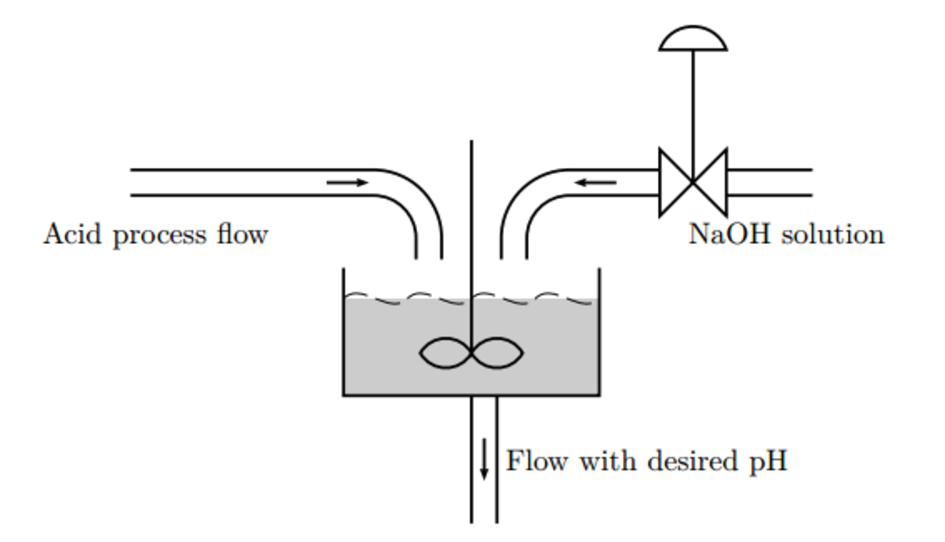
\includegraphics[width=0.5\textwidth]{syratank}
  \caption{Syratank}
  \label{fig:syratank}
\end{figure}

$y(t)$ - pH värdet i utflödet \\
$u(t)$ - Inflödet av NaOH \\
$v(t)$ - Inflödet av syra \\

\textit{Linjärt?} - Troligen inte (otrivial strömning under omrörningen) \\
\textit{Tids-invariant?} - Troligen inte (möjligt att strömningen som uppstår utav omrörningen är tidsberoende) \\
\textit{Kausalt?} - Ja! (fysikaliskt system) \\
\textit{SISO?} - Ja! (en insignal, en utsignal)

\subsection*{b)}

\begin{tikzpicture}[auto, node distance=2cm, >=latex']
\node [block] (system) {Tank};

\draw [wire] (system) -- ++(3,0) node[anchor=base, label={[laba]above:$y(t)$}] {};
\draw [wire] ++(-3,0) node[anchor=base, label={[laba]above:$u(t)$}] {} -- (system);
\draw [wire] ++(0,2) -- (system) node[pos=0.25, right, align=center, label={right:$v(t)$}] {};
\end{tikzpicture}

Ifall $v(t)$ är mätbar kan vi använda \textit{Framkoppling}

\begin{tikzpicture}[auto, node distance=2cm, >=latex']
\node [block] (system) {Tank};
\node [block, left of=system, node distance=4cm] (reg) {Regulator};
\node [split, above of=system, node distance=1.5cm] (split) {};

\draw [wire] (system) -- ++(2,0) node[pos=0.45, right, align=center, label={[laba]below:$y(t)$}] {};
\draw [wire] (reg) -- (system) node[pos=0.45, right, align=center, label={[laba]below:$u(t)$}] {};
\draw [wire] ++(0,2) -- (system) node[pos=0.25, right, align=center, label={right:$v(t)$}] {};
\draw [wire] (split) -| (reg);
\end{tikzpicture}

Med framkoppling kan vi ibland helt eliminera störsignalen (mer om detta i kapitel 7).
\begin{itemize}
\item[$+$] Reagerar snabbt på ändringar i $v(t)$ 
\item[$-$] Kräver att $v(t)$ är mätbar
\item[$-$] Känslig för modellfel, kräver god information om processen
\end{itemize}

Ifall $v(t)$ inte går att mäta använder vi \textit{Negativ återkoppling}

\begin{tikzpicture}[auto, node distance=2cm, >=latex']
\node [block] (system) {Tank};
\node [block, left of=system, node distance=4cm] (reg) {Regulator};
\node [split, right of=system] (split) {};
\node [sum, left of=reg, node distance=3cm] (sum) {};
\node [tmp, below of=reg] (tmp){};

\draw [wire] ++(-9,0) -- node[pos=0.99] {$+$} (sum) node[pos=0.45, right, align=center, label={[laba]below:$y_{ref}(t)$}] {};
\draw [wire] (sum) -- (reg) node[pos=0.45, right, align=center, label={[laba]below:$e(t)$}] {};
\draw [wire] (system) -- ++(4,0) node[pos=0.45, right, align=center, label={[laba]below:$y(t)$}] {};
\draw [wire] (reg) -- (system) node[pos=0.45, right, align=center, label={[laba]below:$u(t)$}] {};
\draw [wire] ++(0,2) -- (system) node[pos=0.25, right, align=center, label={right:$v(t)$}] {};
\draw [wire] (split) |- (tmp) -| node[pos=0.99, right] {$-$} (sum);
\end{tikzpicture}

Den här typen av reglering är vanligast i den här kursen.

\begin{itemize}
\item[$+$] Kan stabilisera instabila system
\item[$+$] Behöver inte mäta $v(t)$ för att dämpa störningen
\item[$-$] Långsammare störningsdämpning än framkoppling
\item[$-$] Känslig för mätbrus i $y(t)$
\end{itemize}

\section*{Teori}

Differentialekvationen \eqref{eq:dynsys} har känd analytisk lösning

\begin{equation*}
y(t) = y_0 e^{-at}
\end{equation*}

\begin{figure}[h!]
  \centering
  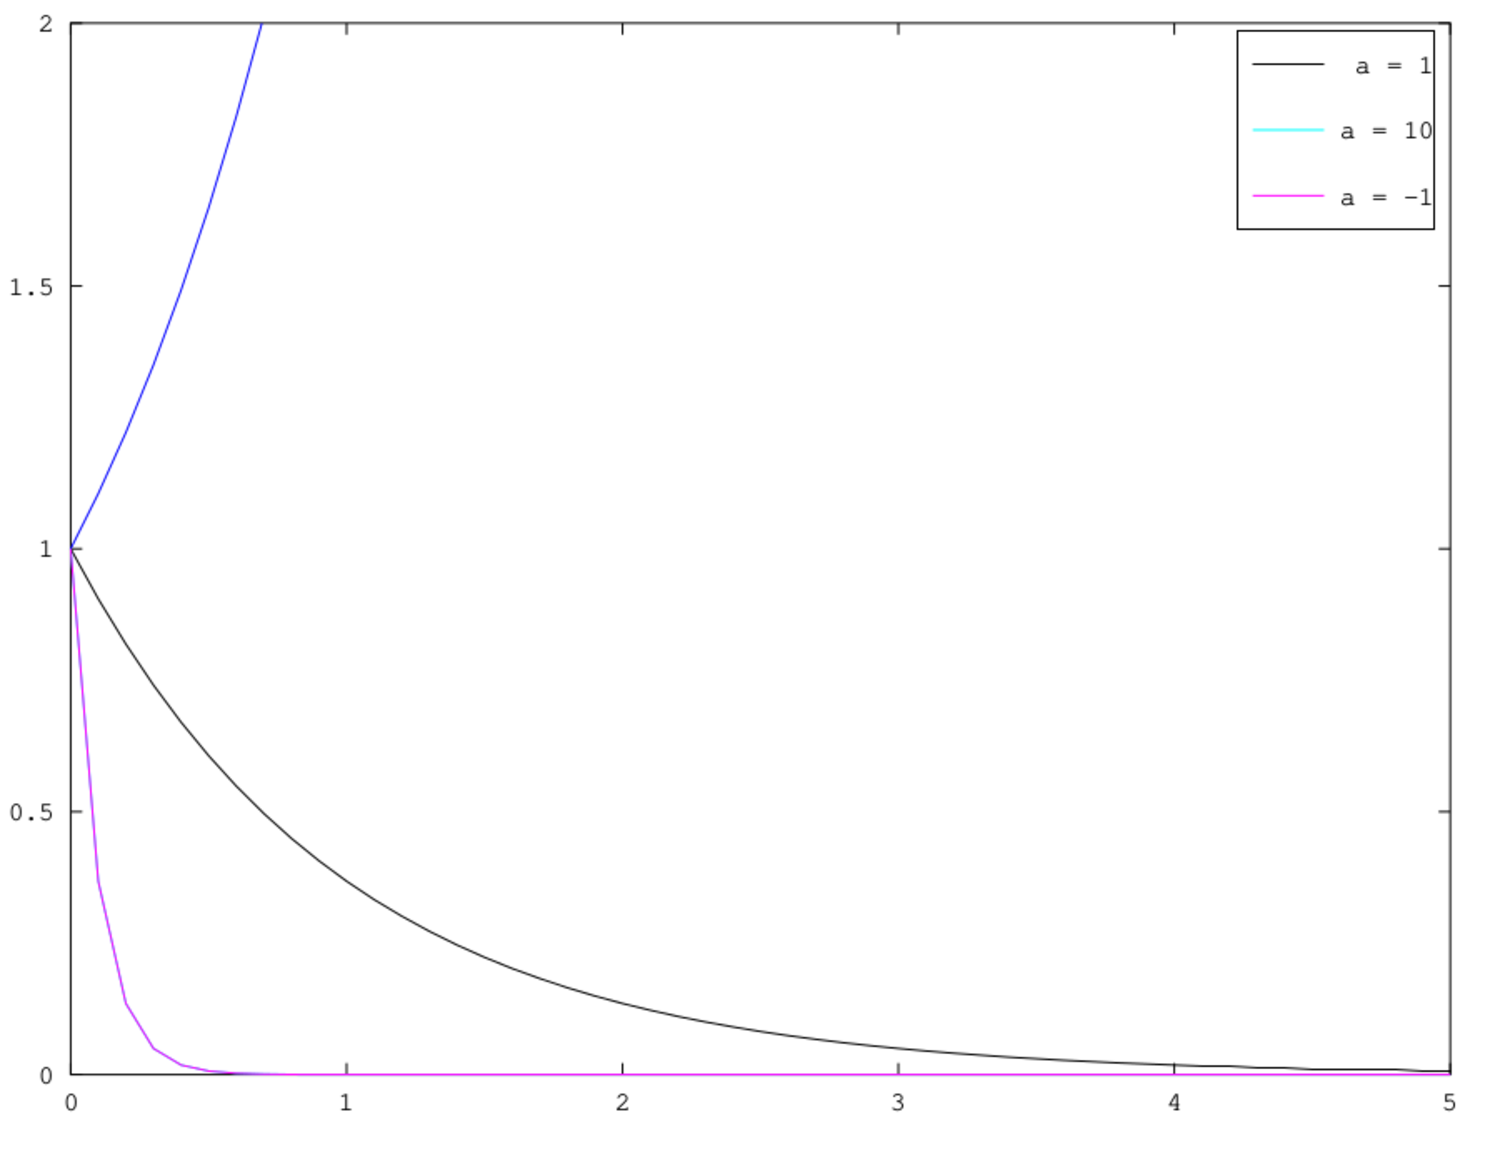
\includegraphics[width=\textwidth]{dynsys}
  \caption{Solutions to \eqref{eq:dynsys} for different values of $a$}
  \label{fig:dynsys}
\end{figure}
\FloatBarrier
Det är tydligt att parametern $a$ styr huruvida lösningen divergerar eller avtar. Storleken på $a$ styr även hur snabbt lösningen går mot noll/oändligheten. Mer involverade differentialekvationer går ej att lösa analytiskt, men vi kommer kunna dra liknande slutsatser om stabilitet och snabbhet via andra metoder.

\textbf{Laplacetransformen}
\begin{equation*}
\mathcal{L}[y(t)] = \int_{0}^{\infty}y(t)e^{-st}\mathrm{d}t := Y(s)
\end{equation*}
(Kommer ofta användas som verktyg under kursens gång, repetera!) \\
\textbf{Överföringsfunktion} \\
''Överför en signal till en annan i Laplacedomänen'' \\
\begin{equation*}
  Y(s) = G(s)U(s)
\end{equation*}
Ex) \\
\begin{equation*}
  \dot{y}(t) = -ay(t) + u(t)
\end{equation*}
Antag att $y(0) = 0$ (systemet är inledningsvis i vila) och laplacetransformera:
\begin{align*}
  sY(s) &= -aY(s) + U(S) \\
\Rightarrow Y(s) &= \frac{1}{s+a}U(s) \\
\Rightarrow G(s) &= \frac{1}{s+a}
\end{align*}
Notera att överföringsfunktionen har ett polynom i nämnaren; detta gäller allmänt för linjära system!

\fbox{\parbox{\textwidth}{
För linjära system
  \begin{itemize}
  \item $G(s) = \dfrac{P(s)}{Q(s)}$ där $P(s)$, $Q(s)$ polynom
  \item \textit{Pol}: Nollställe till $Q(s)$, singularitet till $G(s)$
  \item \textit{Nollställe}: Nollställe till $P(s)$
  \end{itemize}
}}

Poler är viktiga för stabilitet. Deras position i komplexa talplanet avgör ifall ett linjärt system är stabilt eller inte
\begin{itemize}
\item Poler strikt i vänster halvplan $\Leftrightarrow$ insignal-utsignal stabilt system
\item Poler strikt i höger halvplan $\Leftrightarrow$ instabilt system
\item Polernas avstånd från origo avgör hur snabbt systemet är 
\item Poler med imaginärdel ger upphov till svängningar
\end{itemize}
(insignal-utsignal stabilt: begränsade insignaler ger begränsade utsignaler) \\\\
Ex) \\
Överföringsfunktionen motsvarande \eqref{eq:dynsys} har nämnarpolynomet $Q(s) = s+a$ och således en pol i $s = -a$. Enligt ovan är systemet stabilt för $a > 0$ och instabilt för $a < 0$ vilket stämmer överens med lösningarna i figur \ref{fig:dynsys}. \\

Nollställen är viktiga för ett systems \textit{transienta} egenskaper $\rightarrow$ spelar stor roll för styrningen. \\

\textbf{Stegsvar} \\
Utsignalen då insignalen är ett enhetssteg, dvs
\begin{equation*}
  u(t) = \begin{cases}
0, t < 0 \\
1, t >= 0
\end{cases}
\end{equation*}
Analys av stegsvaret ger information om ett systems egenskaper. \\

\textbf{Slutvärdessatsen} \\
Ifall $sY(s)$ saknar singularitet (stabilt system) så gäller att
\begin{equation}
  \label{eq:fvtheorem}
  \lim_{t \to \infty}y(t) = \lim_{s \to 0}sY(s)
\end{equation}
Med slutvärdessatsen kan systemets transient undersökas utan att explicit lösa ut $y(t)$!. \\

\textbf{Statisk förstärkning} \\
\begin{equation*}
  Y(s) = G(s)U(s) = \frac{G(s)}{s} \text{   (stegsvar)}
\end{equation*}
\begin{equation*}
  \Rightarrow \lim_{t \to \infty} y(t) = \lim_{s \to 0}sY(s) = \lim_{s \to 0} s \frac{G(s)}{s} = G(0)
\end{equation*}
$\Rightarrow |G(0)|$ - statisk förstärkning av en konstant insignal.

\section*{Uppgift 2.5}

Para ihop varje pol-nollställe diagram med motsvarande stegsvar.

\begin{figure}[h!]
  \centering
  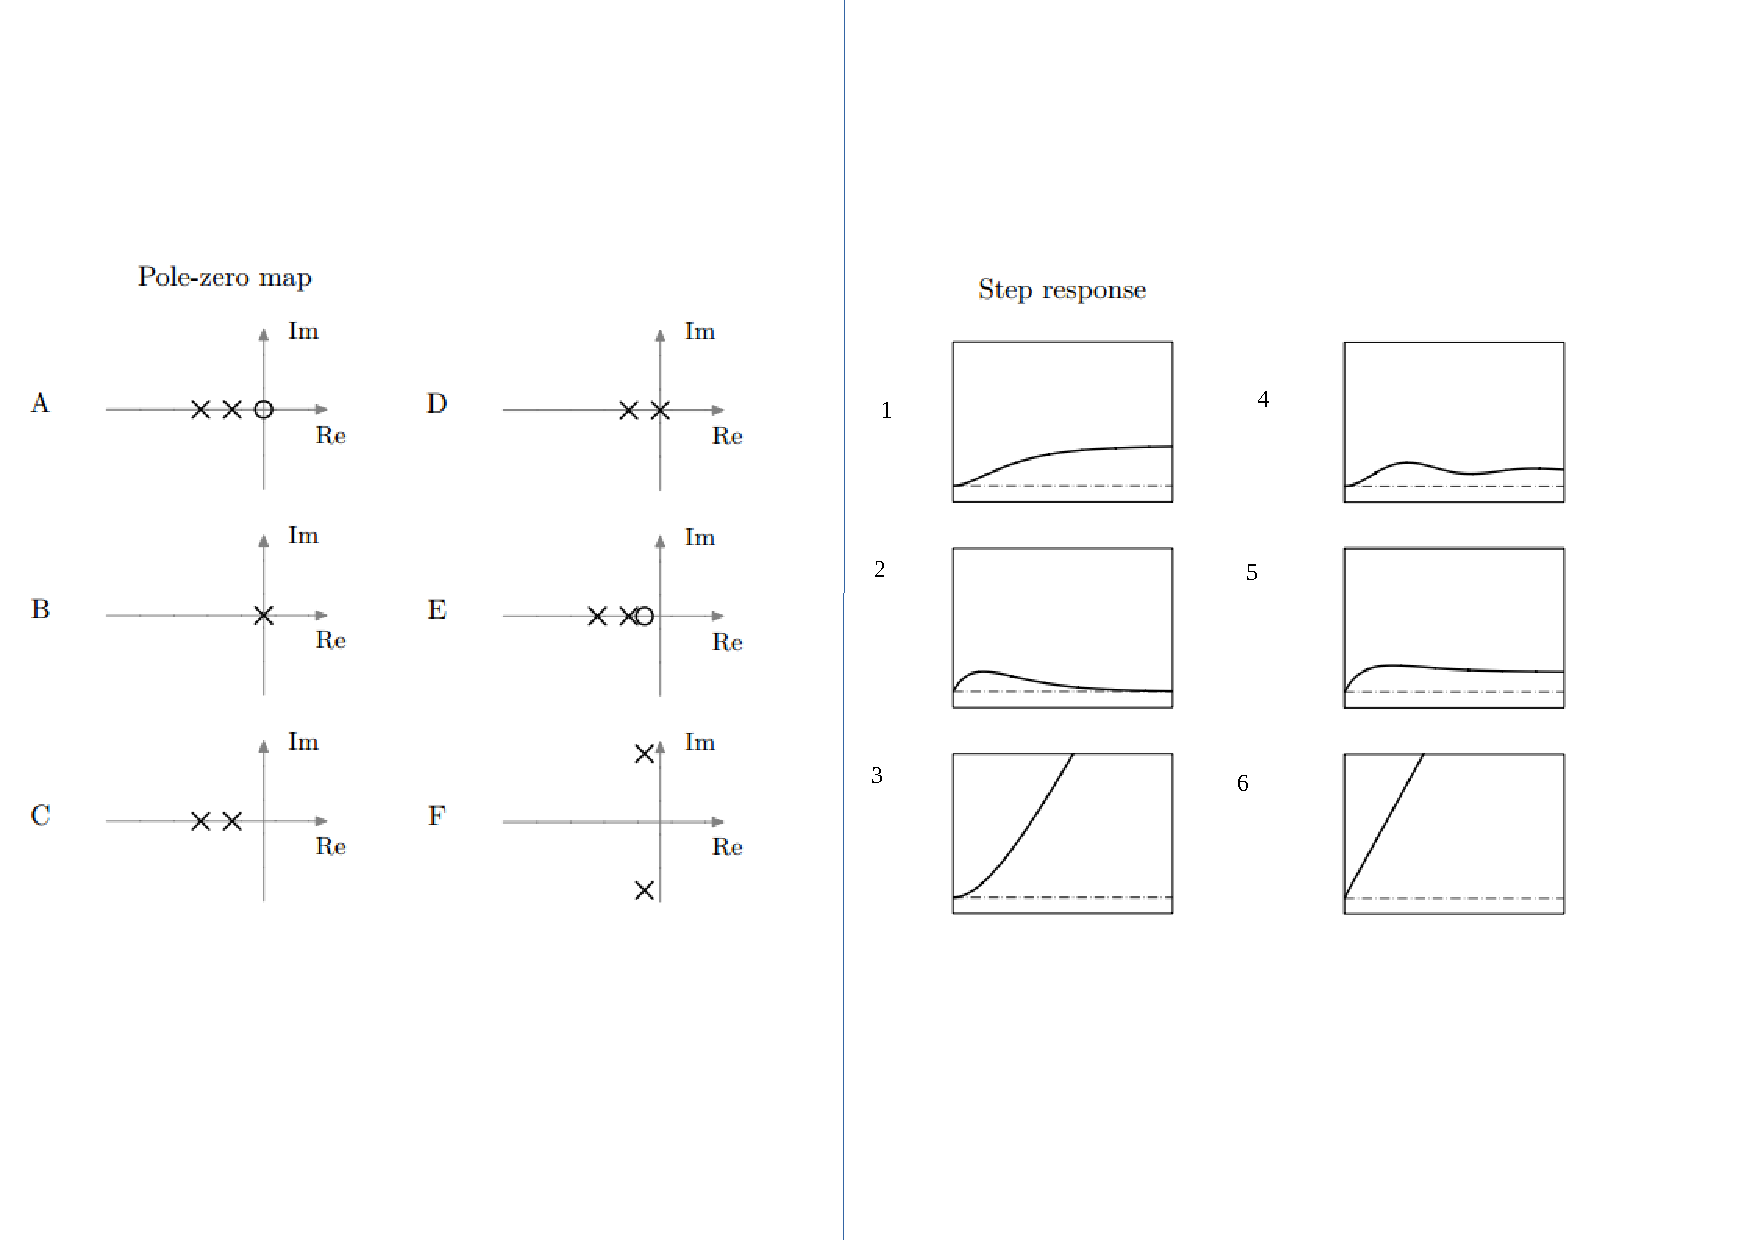
\includegraphics[width=\textwidth]{2_5}
  \caption{Bokstaverade pol-nollställe diagram samt numrerade stegsvar}
  \label{fig:exercise25}
\end{figure}
\FloatBarrier

Stegsvar 3 och 6 divergerar, vilket tyder på instabilitet. Diagram B och D har båda varsin pol i origo, medan de andra systemen har poler strikt i VHP. \\
$\Rightarrow$ B,D $\leftrightarrow$ 3,6 \\

Hur kan vi skilja B och D åt? \\
B har en pol i origo, alltså gäller
\[G_B = \frac{1}{s} \Rightarrow Y(S) = \frac{1}{s}U(s) \Rightarrow sY(s) = U(s)\]
\[\Rightarrow \dot{y}(t) = u(t) \]
Ifall $u(t)$ är ett enhetssteg (konstant signal) så blir även $\dot{y(t)}$ konstant. Stegsvar 6 har konstant lutning. Alltså gäller \\
B $\leftrightarrow$ 6 \\
D $\leftrightarrow$ 3 \\\\
F är det enda systemet med komplexa poler och stegsvar 4 är det enda stegsvaret som uppvisar svängigt beteende. \\
F $\leftrightarrow$ 4 \\\\
A har ett nollställe i origo 
\[G_A (s) = \frac{s}{(s+a)(s+b)}\]
\[\lim_{t \to \infty} y(t) = \lim_{s \to 0} sG_A (s) U(s) = \lim_{s \to 0} s \cdot \frac{s}{(s+a)(s+b)} \cdot \frac{1}{s} = 0\]
Endast stegsvar 2 går mot noll i stationäritet. Alltså gäller \\
A $\leftrightarrow$ 2 \\\\
C,E är båda stabila, men E har ett nollställe.
\[G_c(s) = \frac{1}{(s+a)(s+b)} \Rightarrow Y_c (s) = \frac{1}{(s+a)(s+b)} \cdot \frac{1}{s} \text{ (stegsvar)}\]
\[\Rightarrow y_c (t) = \lbrace \text{från laplace tabell} \rbrace = \frac{1}{ab} \left(1 - \frac{be^{-at}-ae^{-bt}}{b-a}\right)\]
\[\Rightarrow \dot{y}_c(t) = \frac{e^{-at} - e^{-bt}}{b-a}\]
\[\Rightarrow \dot{y}_c(t) = 0 \Leftrightarrow e^{(a-b)t} = 1 \]
Men $a \neq b$, så enbart $\dot{y}_c (0) = 0$ gäller. Alltså innehåller stegsvaret till C ingen översläng! Således gäller \\
C $\leftrightarrow$ 1 \\
E $\leftrightarrow$ 5 \\\\
\textbf{Sammanfattningsvis:} \\
B $\leftrightarrow$ 6 \\
D $\leftrightarrow$ 3 \\
F $\leftrightarrow$ 4 \\
A $\leftrightarrow$ 2 \\
C $\leftrightarrow$ 1 \\
E $\leftrightarrow$ 5 \\

\section*{Uppgift 2.10}
\begin{figure}[h!]
  \centering
  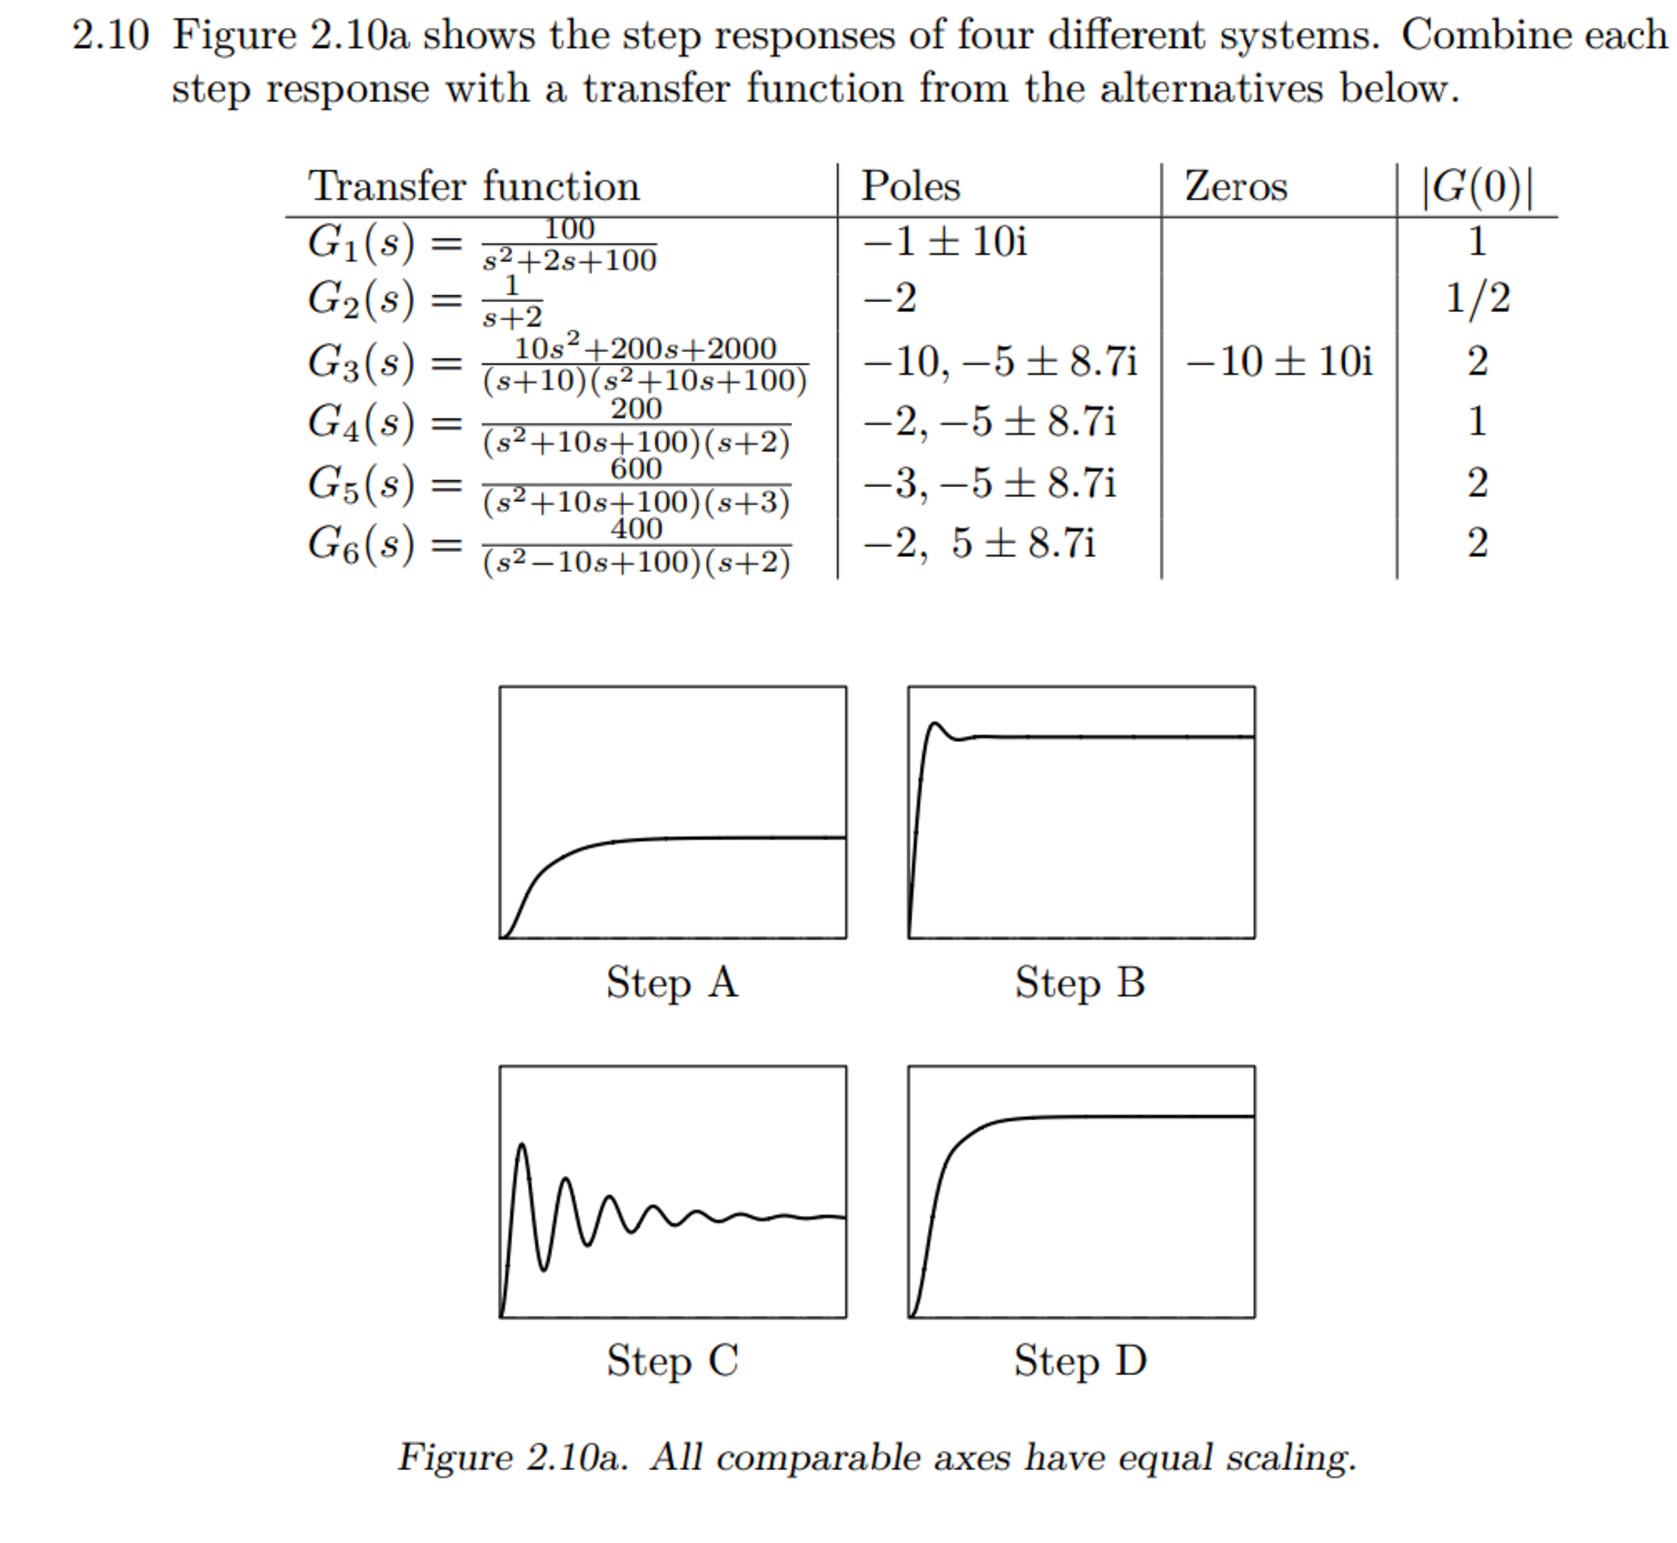
\includegraphics[width=0.7\textwidth]{2_10}
\end{figure}
\FloatBarrier

Alla stegsvar är stabila. $G_6(s)$ har poler i HHP \\
$\Rightarrow$ uteslut $G_6(s)$ \\\\
B,D har dubbel statisk förstärkning som A,C. Enda konfigurationen när detta är möjligt (notera överföringsfunktionernas statiska förstärlning) är ifall \\
$G_1(s), G_4(s)$ $\leftrightarrow$ A,C \\
$G_3(s), G_5(s)$ $\leftrightarrow$ B,D \\
$\Rightarrow$ uteslut $G_2(s)$ \\\\
$G_4(s)$ har pol i $-2$ som dominerar det komplexa polparet i $-5 \pm 8.7i$. $G_1(s)$ får svag dämpning som följd av det komplexa polparet med stor imaginärdel $-1 \pm 10i$. Därav följer att \\
$G_1(s)$ $\leftrightarrow$ C \\
$G_4(s)$ $\leftrightarrow$ A \\\\
$G_3(s)$ har ett nollställe och polen i $-10$ är markant större än $G_5(s)$:s pol i $-1$ vilket indikerar att $G_3(s)$ kommer ge ett snabbare stegsvar (med risk för översläng). Därav följer att
$G_3(s)$ $\leftrightarrow$ B \\
$G_5(S)$ $\leftrightarrow$ D \\\\
\textbf{Sammanfattningsvis:} \\
$G_1(s)$ $\leftrightarrow$ C \\
$G_4(s)$ $\leftrightarrow$ A \\
$G_3(s)$ $\leftrightarrow$ B \\
$G_5(s)$ $\leftrightarrow$ D \\
\end{document}
